% http://guitarpenguin.is-programmer.com/posts/48869.html
\documentclass{article}
\def\pgfsysdriver{pgfsys-tex4ht.def}
%There is specialized output driver for use with tex4ht in Tikz. Using it, diagrams are saved in SVG.
\usepackage{tikz}
\usepackage{pgf}
\usetikzlibrary{automata}
\usetikzlibrary{positioning,chains,fit,shapes,calc}
\usetikzlibrary{arrows,shadows,trees}
\begin{document}
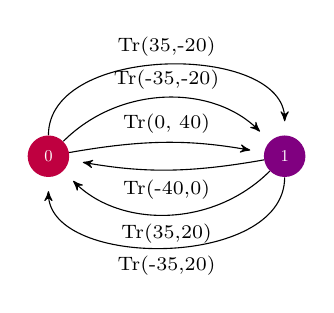
\begin{tikzpicture}[->,>=stealth',shorten >=5pt,auto,node distance=1cm]
\tikzstyle{every state}=[fill=purple, draw=none, text=white]
\node[state, scale=0.6] (A) at (0,0) {$0$};
\node[state, scale=0.6, fill=violet] (B) at (3,0) {$1$};
\path (A) edge [bend left=10] node {\scriptsize{Tr(0, 40)}} (B)
      (A) edge [bend left=45] node {\scriptsize{Tr(-35,-20)}} (B)
      (A) edge [bend left=90] node {\scriptsize{Tr(35,-20)}} (B)
      (B) edge [bend left=10] node {\scriptsize{Tr(-40,0)}} (A)
      (B) edge [bend left=45] node {\scriptsize{Tr(35,20)}} (A)
      (B) edge [bend left=90] node {\scriptsize{Tr(-35,20)}} (A);
\end{tikzpicture}
\end{document}
